% 자동 생성: scripts/plot_composite_final_dist.py — 수정은 스크립트에서
% 데이터: composite-final-20260814T114929Z cases.jsonl (r_total, n={'seq2': 500, 'pool': 500})
\documentclass[tikz,border=2pt]{standalone}
\usepackage{pgfplots}
\pgfplotsset{compat=1.18}
\definecolor{seqblue}{HTML}{3A6FE0}
\definecolor{poolred}{HTML}{D5484A}
\begin{document}
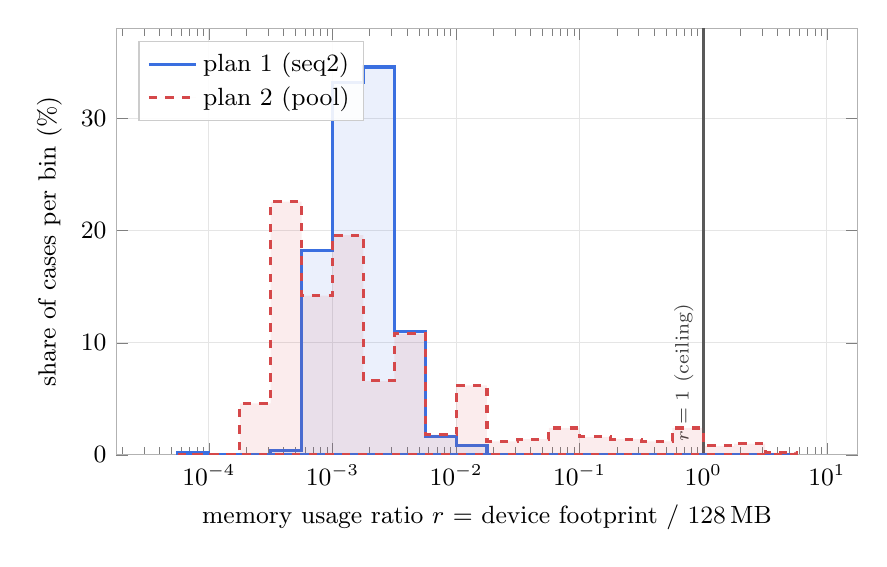
\begin{tikzpicture}
\begin{axis}[
  width=11cm, height=7cm,
  xmode=log,
  xlabel={memory usage ratio $r$ = device footprint / 128\,MB},
  ylabel={share of cases per bin (\%)},
  ymin=0,
  grid=major, grid style={gray!20},
  axis line style={gray!60},
  tick label style={font=\small},
  label style={font=\small},
  legend style={at={(0.03,0.97)}, anchor=north west, font=\small,
                 draw=gray!40, fill=white, fill opacity=0.9, text opacity=1},
  legend cell align=left,
]
\draw[black!65, line width=0.9pt] (axis cs:1,0) -- (axis cs:1,\pgfkeysvalueof{/pgfplots/ymax});
\node[gray!50!black, font=\scriptsize, anchor=south west, rotate=90]
  at (axis cs:1,0.3) {$r=1$ (ceiling)};
\addplot[seqblue, solid, line width=1.1pt, const plot,
  fill=seqblue, fill opacity=0.10, draw opacity=1] coordinates {
(5.62341e-05,0.200)(0.0001,0.000)(0.000177828,0.000)(0.000316228,0.400)(0.000562341,18.200)
(0.001,33.200)(0.00177828,34.600)(0.00316228,11.000)(0.00562341,1.600)(0.01,0.800)
(0.0177828,0.000)(0.0316228,0.000)(0.0562341,0.000)(0.1,0.000)(0.177828,0.000)
(0.316228,0.000)(0.562341,0.000)(1,0.000)(1.77828,0.000)(3.16228,0.000)
(5.62341,0.000)} \closedcycle;
\addlegendentry{plan 1 (seq2)}
\addplot[poolred, dashed, line width=1.1pt, const plot,
  fill=poolred, fill opacity=0.10, draw opacity=1] coordinates {
(5.62341e-05,0.000)(0.0001,0.000)(0.000177828,4.600)(0.000316228,22.600)(0.000562341,14.200)
(0.001,19.600)(0.00177828,6.600)(0.00316228,10.800)(0.00562341,1.800)(0.01,6.200)
(0.0177828,1.200)(0.0316228,1.400)(0.0562341,2.400)(0.1,1.600)(0.177828,1.400)
(0.316228,1.200)(0.562341,2.400)(1,0.800)(1.77828,1.000)(3.16228,0.200)
(5.62341,0.200)} \closedcycle;
\addlegendentry{plan 2 (pool)}
\end{axis}
\end{tikzpicture}
\end{document}
